%TP genérico



%Configuracion del documento

%Tamaño de letra principal:

\documentclass[12pt]{article}


%Título y autor(es):

\title{Red de Hopfield}
\author{Sergio}


%Tamaño de página y los márgenes:
\usepackage[a4paper,headheight=16pt]{geometry}

\textwidth      =  450pt     %Ancho del cuerpo
\textheight     =  650pt     %Largo del cuerpo
\topmargin      =  0pt       %Agrega espacio en el margen superior
\oddsidemargin  =  0pt       %+ margen izquierdo en paginas impares
\evensidemargin =  0pt       %+ margen derecho en paginas impares


% castellano:
\usepackage[spanish]{babel}

%instalar texlive-lang-spanish
% Reconocer acentos y caracteres no ingleses:

\usepackage[utf8]{inputenc}


% Cabecera y pie de página personalizadas
\usepackage{fancyhdr}
\pagestyle{fancy}

% Hago que en la cabecera de página se muestre a la derecha la sección,
% y en el pie, en número de página a la derecha:

\renewcommand{\sectionmark}[1]{\markboth{}{\thesection\ \ #1}}
\lhead{}
\chead{}
\rhead{\rightmark}
\lfoot{}
\cfoot{}
\rfoot{\thepage}


%numeracion especial para tablas, figuras y ecuaciones
\usepackage{amsmath}
\numberwithin{equation}{section}
\numberwithin{figure}{section}
\numberwithin{table}{section}


%Agregar notas al pie en tablas:
\usepackage{threeparttable}


%Incluir Graficos
\usepackage{graphicx}


%Usar subfiguras: (al estilo Figura 2.3(b) )
\usepackage{subfigure}
\usepackage{float}

% Para esto es necesario texlive-latex-recommended o texlive-latex-extra

%Numero de figuras en negrita
\usepackage[hang,bf]{caption}


% Todas las imágenes están en el directorio tp-img:
\newcommand{\imgdir}{img}
\graphicspath{{\imgdir/}}

% uso de colores
\usepackage{color}
\definecolor{light-gray}{gray}{0.95}

%Para embeber código de lenguajes como Matlab, C, html, etc.

\usepackage{listings}
\lstset{ frame=Ltb, 
	framerule=0pt, 
	aboveskip=0.5cm, 
	%framextopmargin=3pt, 
	%framexbottommargin=3pt, 
	%framexleftmargin=0.4cm, 
	framesep=3pt, rulesep=.4pt, 
	backgroundcolor=\color{light-gray}, 
	rulesepcolor=\color{black}, 
	showstringspaces = false, 
	basicstyle=\small\ttfamily, 
	commentstyle=\color{green}, 
	keywordstyle=\bfseries,
	numbers=left
	}


	%rulesepcolor=\color{black},
	%stringstyle=\ttfamily,
	%showstringspaces = false,
	%basicstyle=\small\ttfamily,
	%commentstyle=\color{gray},
	%keywordstyle=\bfseries,

	%numbers=left,
	%numbersep=15pt,
	%numberstyle=\tiny,
	%numberfirstline = false,
	%breaklines=true


%Para colocar hipervinculos

\usepackage[colorlinks=true,linkcolor=black,urlcolor=blue]{hyperref}

%Para hacer matrices y digramas de flujo sencillos

%\usepackage[all]{xy}
\usepackage{pdfpages}


%INICIO DEL DOCUMENTO

%-------------------------------------------------------------------------------



\begin{document}



% CARATULA

%-------------------------------------------------------------------------------



\begin{titlepage}

% Sin cabecera ni pie de página:

\thispagestyle{empty}



% Logo de la facu: 

	
\includegraphics[width=5cm]{logo-facu}

\vfill



% Título:

\begin{center}
	\Huge{Descripción de objetos}\\

\end{center}

\vspace{4cm}



% Integrantes:

\large{

	\begin{tabbing}
		Sergio Hinojosa \hspace{1cm} \\84476 \\
	\end{tabbing}

}

\vfill

% Fecha o cuatrimestre:

%\flushright{2012}

\end{titlepage}




% Hago que las páginas se comiencen a contar a partir de aquí:

\setcounter{page}{1}



%INDICE

%-------------------------------------------------------------------------------

% Pongo el índice en una página aparte:

%\tableofcontents

%\newpage



%-------------------------------------------------------------------------------


% Inicio del TP:
\section{NeuroDB}

\begin{figure}[H]
	\centering
	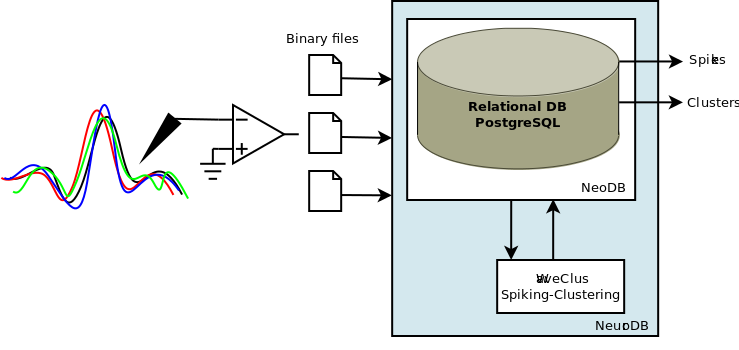
\includegraphics[width=14cm]{neurodb.png}
	\caption{}
	\label{fig:neurodb}
\end{figure}



\begin{figure}[H]
	\centering
	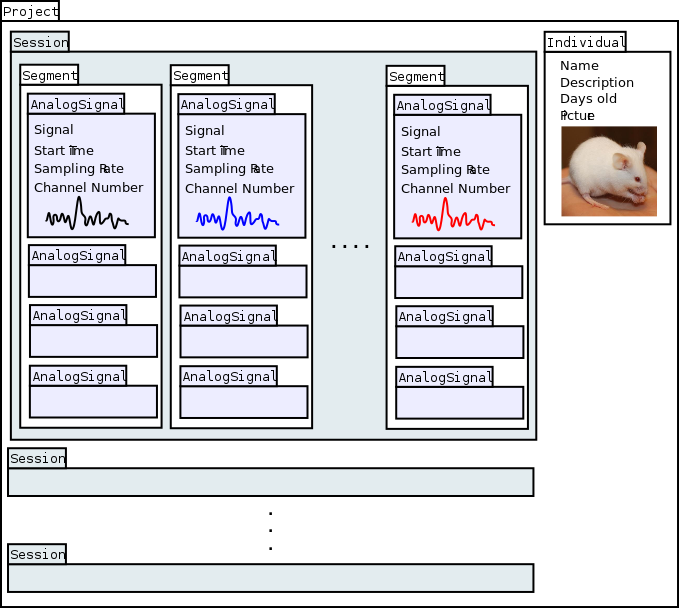
\includegraphics[width=14cm]{project.png}
	\caption{}
	\label{fig:neurodb}
\end{figure}

\subsubsection*{create\_project(name,date,description,index)}
Genera una entrada en la tabla project correspondiente a un nuevo proyecto. En caso de existir un proyecto con el mismo nombre e index (si existe) se lanza una excepción.

\subsubsection*{create\_individual(name,description,picture\_path,days\_old)}
Genera una entrada en la tabla individual correspondiente a un nuevo individuo sujeto de experimentación. En caso de existir un individuo con el mismo nombre se lanza una excepción. "picture\_path" corresponde al path donde se encuentra la imagen del individuo, no es un parámetro obligatorio, en caso de no ser válido se lanza una excepción.

\subsubsection*{create\_session(id\_project,id\_individual,rec\_datetime,name,description)}
Genera una entrada en la tabla block correspondiente a un nueva sesión de registro.
id\_project e id\_individual son obligatorios.

\subsubsection*{save\_segment(id\_session,filename,t\_start,sampling\_rate,nchannels,dtype,description)}
Procesa el archivo parcial de los registros. Genera una entrada en la tabla segment y una entrada por cada segmento de señal de cada canal en la tabla analogsignal. El único parámetro no obligatorio es description.

\subsubsection*{connect\_db(host,user,password,dbname)}
Genera la conexión a la base, ninguno de los anteriores métodos funciona sin antes haber llamado a esta función.

\subsubsection*{create\_db(host,user,password,dbname)}
Crea las tablas del sistema, en caso de existir lanza una excepción.


\subsection*{NeoDB}
Basado en el paquete Neo de Python, se implementa el paquete NeoDB para la implementación de la base de datos propuesta, con la posibilidad de generar a partir de los objetos de NeoDB.core objetos Neo para ser utilizados en los programas que soportan esta representación de datos.



\end{document}
